\documentclass{beamer}
\usetheme{Antibes}
\usepackage{xcolor, colortbl}
\usepackage{algorithm}
\usepackage{algpseudocode}
\usepackage{textcomp}
\usepackage{listings}
\usepackage{hyperref}
\usepackage{alltt}
\usepackage{tikz}
\usepackage{framed}
\usepackage{marvosym}
\usepackage{wasysym}
\usepackage{marvosym}
\usepackage{crayola}
\usepackage{mathpartir}
\usepackage{tabularx}
\usepackage[belowskip=-15pt,aboveskip=0pt]{caption}
\usepackage[skins]{tcolorbox}
\usepackage{multicol}
\usetikzlibrary{positioning,shapes,arrows, backgrounds, fit, shadows, automata}
\usetikzlibrary{decorations.markings, calc}
%\usepackage{wasysym}
%\usepackage{marvosym}
\setbeamertemplate{footline}[frame number]
%\usecolortheme{fly}
\usefonttheme{serif}

\title[Sujit]{Lexical Analysis \\
Programming Languages}
\author{Sujit Kumar Chakrabarti}
\institute{IIITB}
\date{}


\definecolor{lightblue}{rgb}{0.8,0.93,1.0} % color values Red, Green, Blue
\definecolor{darkblue}{rgb}{0.4,0.3,1.0} % color values Red, Green, Blue
\definecolor{Blue}{rgb}{0,0,1.0} % color values Red, Green, Blue
\definecolor{darkgreen}{rgb}{0,0.7,0.2} % color values Red, Green, Blue
\definecolor{Red}{rgb}{1,0,0} % color values Red, Green, Blue
\definecolor{Pink}{rgb}{0.7,0,0.2}
\definecolor{links}{HTML}{2A1B81}
\definecolor{mydarkgreen}{HTML}{126215}
\newcommand{\highlight}[1]{{\color{Red}(#1)}}

\newcommand{\myheader}[1]{
	{\color{darkblue}
		\begin{Large}
			\begin{center}
				{#1}
			\end{center}
		\end{Large}
	}
}
\newcommand{\myminorheader}[1]{
	{\color{BrickRed}
		\begin{Large}
			{\fontfamily{\sfdefault}\selectfont\textbf{#1}}
		\end{Large}
	}
}

%\tikzstyle{input} = [coordinate]
%\tikzstyle{output} = [coordinate]


\tikzstyle{bb}=[%
      rectangle, draw=black, thick, fill=OliveGreen!30, drop shadow, align=center,
      text ragged, minimum height=2em, minimum width=2em, inner sep=6pt
]

\tikzstyle{inv}=[%
      rectangle, draw=none,  align=center,
      text ragged, minimum height=2em, minimum width=2em, align=center, inner sep=6pt
]

\tikzstyle{db}=[%
      ellipse, draw=black, thick, fill=pink, drop shadow, align=center,
      text ragged, minimum height=2em, inner sep=6pt
]

\tikzstyle{jn}=[%
      inner sep=0cm, outer sep=0cm
]

\tikzstyle{io}=[%
      trapezium, trapezium left angle=60, trapezium right angle=120, draw=black, thick, fill=brown, drop shadow,
      text ragged, minimum height=2em, minimum width=2em, inner sep=6pt, align=center
]

\tikzstyle{glio}=[%
      trapezium, trapezium left angle=60, trapezium right angle=120, draw=red, line width = 1mm, fill=brown, drop shadow,
      text ragged, minimum height=2em, minimum width=2em, inner sep=6pt
]
\tikzstyle{gl}=[%
      rectangle, draw=red, line width = 1mm, fill=lightblue, drop shadow,
      text ragged, minimum height=2em, minimum width=2em, inner sep=6pt
]

\tikzstyle{en}=[%
      rectangle, draw=black, thick, fill=none,
      text ragged, minimum height=2em, minimum width=2em, inner sep=6pt
]

\tikzstyle{sh}=[%
      rectangle, draw=gray, thick, fill=none, color = gray,
      text ragged, minimum height=2em, minimum width=2em, inner sep=6pt
]


\lstdefinestyle{javacode}{
	language = Java,
	basicstyle = \ttfamily\scriptsize,
	stringstyle = \ttfamily,
	keywordstyle=\color{Blue}\bfseries,
	identifierstyle=\color{Pink},
	commentstyle=\color{darkgreen},
	frame=single,
	frameround=tttt,
%	numbers=left
	showstringspaces=false
}

\lstdefinestyle{camlcode}{
	language = Caml,
	basicstyle = \scriptsize\ttfamily,
	stringstyle = \color{red}\ttfamily,
	keywordstyle=\color{Blue}\bfseries,
	identifierstyle=\ttfamily,
	frame=single,
	frameround=tttt,
	numbers=none,
	showstringspaces=false,
	escapeinside={(*@}{@*)}
}

\lstdefinestyle{outputcode}{
	language = bash,
	backgroundcolor = \color{black},
	basicstyle = \tiny\ttfamily\color{white},
	stringstyle = \color{red}\ttfamily,
	keywordstyle=\color{white}\bfseries,
	identifierstyle=\ttfamily,
	frameround=tttt,
	numbers=none,
	showstringspaces=false,
	escapeinside={(*@}{@*)}
}

\newtcolorbox{myframe}[2][]{%
  enhanced,colback=white,colframe=black,coltitle=black,
  sharp corners,boxrule=0.4pt,
  fonttitle=\itshape,
  attach boxed title to top left={yshift=-0.3\baselineskip-0.4pt,xshift=2mm},
  boxed title style={tile,size=minimal,left=0.5mm,right=0.5mm,
    colback=white,before upper=\strut},
  title=#2,#1
}

\begin{document}
\maketitle

\section{Simulation of FSA}
% frame begin %%%%%%%%%%%%%%%%%%%%%%%%
\begin{frame}{FSA and Lexical Analysis}
\begin{enumerate}
	\item Each token class has an FSA.
	\item FSA acts as the recogniser of a token.
	\item FSA simulated to accept or reject a string.
\end{enumerate}

\pause
FSA simulation is central to lexical analysis.
\end{frame}
% frame end %%%%%%%%%%%%%%%%%%%%%%%%




\section{Simulation of DFAs}


% frame begin %%%%%%%%%%%%%%%%%%%%%%%%
\begin{frame}{Deterministic FSA (DFA)}
\begin{itemize}
	\item Finite set of states -- ($S$)
	\item Alphabet - ($\sum$)
	\item Transition function ($T : S \times \sum \rightarrow S$)
	\item Initial state ($S_0$)
	\item Final/accepting states ($F \subseteq S$)
	\item \textbf{Acceptance of a string: }When there exists a path corresponding to the input leading to an accepting state.
\end{itemize}

\end{frame}
% frame end %%%%%%%%%%%%%%%%%%%%%%%%

% frame begin %%%%%%%%%%%%%%%%%%%%%%%%
\begin{frame}{Simulating FSAs}

\myminorheader{Representating \textit{transition function} using transition tables}
\begin{center}
\resizebox{!}{0.2\textheight}{%
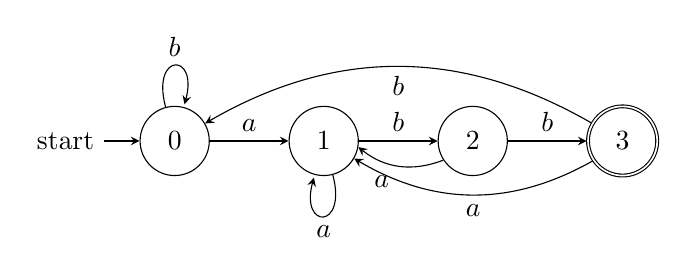
\begin{tikzpicture}[auto,
    ->,
    >=stealth
  ]
    \node[initial, state]   (0)                {$0$};
    \node[state]            (1) [right = of 0] {$1$};
    \node[state] (2) [right = of 1] {$2$};
    \node[state, accepting] (3) [right = of 2] {$3$};
    
    \path (0) edge[loop above] node {$b$} (0)
          (0) edge node {$a$} (1)
          (1) edge[loop below] node {$a$} (1)
          (1) edge node {$b$} (2)
          (2) edge node {$b$} (3)
          (2) edge[bend left] node {$a$} (1.350)
          (3) edge[bend left] node {$a$} (1.330)
          (3) edge[bend right] node {$b$} (0)
    ;
    
  \end{tikzpicture}
}

\end{center}

\textbf{Transition Table:}
\begin{center}
\begin{tabular}{c | c | c }
\hline
\textbf{State} & \textbf{a}        & \textbf{b}     \\
\hline
\onslide<1->0              & \onslide<2->1          & \onslide<2-> 0\\
\onslide<1->1              & \onslide<2->1              & \onslide<2-> 2\\
\onslide<1->2              & \onslide<2->1              & \onslide<2-> 3\\
\onslide<1->3              & \onslide<2->1              & \onslide<2-> 0
\end{tabular}
\end{center}
\end{frame}
% frame end %%%%%%%%%%%%%%%%%%%%%%%%

% frame begin %%%%%%%%%%%%%%%%%%%%%%%%
\begin{frame}{Simulation of DFA}
\footnotesize
\begin{algorithmic}[0]
\Procedure{simDFA}{$D$, $inp$}
  \State $s \gets D.s_0$ \Comment{$D.s_0$: initial state}
  \While{there is input left}
    \State $c \gets$ \Call{nextChar}{}
    \State $s \gets$ $D$.\Call{move}{$s$, $c$} \Comment{Extract next state from transition table}
    \If{$s$ = \textbf{nil}}
      \State \textbf{break}
    \EndIf
  \EndWhile
  \If{$s \in D.F$} \Comment{$D.F$: Final states}
    \State \textbf{return true}
  \Else
    \State \textbf{return} \textbf{false}
  \EndIf
\EndProcedure

\end{algorithmic}

\end{frame}
% frame end %%%%%%%%%%%%%%%%%%%%%%%%

% frame begin %%%%%%%%%%%%%%%%%%%%%%%%
\begin{frame}{Simulation of DFAs}

\myminorheader{Example 1}

\begin{center}
\resizebox{!}{0.2\textheight}{%
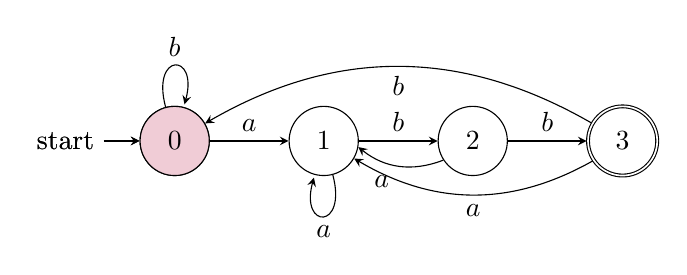
\begin{tikzpicture}[auto,
    ->,
    >=stealth
  ]
    \node[initial, state]   (0)                {$0$};
    \node[state]            (1) [right = of 0] {$1$};
    \node[state] (2) [right = of 1] {$2$};
    \node[state, accepting] (3) [right = of 2] {$3$};
    
    \path (0) edge[loop above] node {$b$} (0)
          (0) edge node {$a$} (1)
          (1) edge[loop below] node {$a$} (1)
          (1) edge node {$b$} (2)
          (2) edge node {$b$} (3)
          (2) edge[bend left] node {$a$} (1.350)
          (3) edge[bend left] node {$a$} (1.330)
          (3) edge[bend right] node {$b$} (0)
    ;
        \node[initial, state, fill=Pink!20]   (0a) at  (0)    {$0$};
  \end{tikzpicture}
}

\vspace{1cm}
\begin{tabular}{p{0.3\textwidth} @{\hspace{1cm}} c}
\textbf{Input:} $aabbabb$ &
\resizebox{0.6\textwidth}{!}{
\begin{tikzpicture}
\node[circle, draw=Black] (s0) {0};
\node[circle, draw=none, right=of s0] (s1) {\ };
\node[circle, draw=none, right=of s1] (s2) {\ };
\node[circle, draw=none, right=of s2] (s3) {\ };
\node[circle, draw=none, right=of s3] (s4) {\ };
\node[circle, draw=none, right=of s4] (s5) {\ };
\node[circle, draw=none, right=of s5] (s6) {\ };
\node[circle, draw=none, right=of s6] (s7) { };

%\draw[->] (s0) to node[above]{a} (s1);
%\draw[->] (s1) to node[above]{a} (s2);
%\draw[->] (s2) to node[above]{b} (s3);
%\draw[->] (s3) to node[above]{b} (s4);
%\draw[->] (s4) to node[above]{a} (s5);
%\draw[->] (s5) to node[above]{b} (s6);
%draw[->] (s6) to node[above]{b} (s7);
\end{tikzpicture}
}
\end{tabular}

\end{center}

\end{frame}
% frame end %%%%%%%%%%%%%%%%%%%%%%%%


% frame begin %%%%%%%%%%%%%%%%%%%%%%%%
\begin{frame}{Simulation of DFAs}

\myminorheader{Example 1}


\begin{center}
\resizebox{!}{0.2\textheight}{%
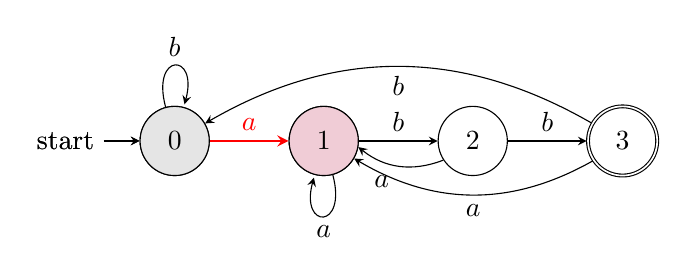
\begin{tikzpicture}[auto,
    ->,
    >=stealth
  ]
    \node[initial, state]   (0)                {$0$};
    \node[state]            (1) [right = of 0] {$1$};
    \node[state] (2) [right = of 1] {$2$};
    \node[state, accepting] (3) [right = of 2] {$3$};
    
    \path (0) edge[loop above] node {$b$} (0)
          (0) edge[Red, thick] node {$a$} (1)
          (1) edge[loop below] node {$a$} (1)
          (1) edge node {$b$} (2)
          (2) edge node {$b$} (3)
          (2) edge[bend left] node {$a$} (1.350)
          (3) edge[bend left] node {$a$} (1.330)
          (3) edge[bend right] node {$b$} (0)
    ;
        \node[state, initial, fill=Gray!20]   (0a) at  (0)    {$0$};
        \node[state, fill=Pink!20]   (1a) at  (1)    {$1$};
  \end{tikzpicture}
}

\vspace{1cm}
\begin{tabular}{p{0.3\textwidth} @{\hspace{1cm}} c}
\textbf{Input:} ${\color{Red}\textbf{a}}abbabb$ &
\resizebox{0.6\textwidth}{!}{
\begin{tikzpicture}
\node[circle, draw=Black] (s0) {0};
\node[circle, draw=Black, right=of s0] (s1) {1};
\node[circle, draw=none, right=of s1] (s2) {\ };
\node[circle, draw=none, right=of s2] (s3) {\ };
\node[circle, draw=none, right=of s3] (s4) {\ };
\node[circle, draw=none, right=of s4] (s5) {\ };
\node[circle, draw=none, right=of s5] (s6) {\ };
\node[circle, draw=none, right=of s6] (s7) { };

\draw[->] (s0) to node[above]{a} (s1);
%\draw[->] (s1) to node[above]{a} (s2);
%\draw[->] (s2) to node[above]{b} (s3);
%\draw[->] (s3) to node[above]{b} (s4);
%\draw[->] (s4) to node[above]{a} (s5);
%\draw[->] (s5) to node[above]{b} (s6);
%draw[->] (s6) to node[above]{b} (s7);
\end{tikzpicture}
}
\end{tabular}

\end{center}

\end{frame}
% frame end %%%%%%%%%%%%%%%%%%%%%%%%

% frame begin %%%%%%%%%%%%%%%%%%%%%%%%
\begin{frame}{Simulation of DFAs}

\myminorheader{Example 1}


\begin{center}
\resizebox{!}{0.2\textheight}{%
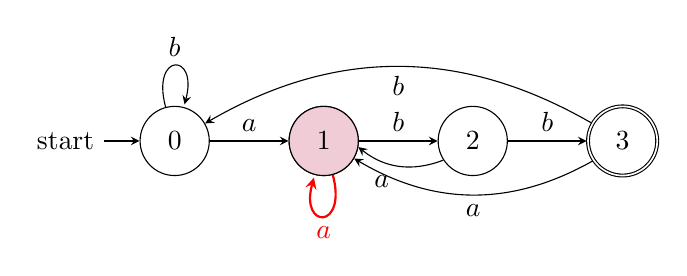
\begin{tikzpicture}[auto,
    ->,
    >=stealth
  ]
    \node[initial, state]   (0)                {$0$};
    \node[state]            (1) [right = of 0] {$1$};
    \node[state] (2) [right = of 1] {$2$};
    \node[state, accepting] (3) [right = of 2] {$3$};
    
    \path (0) edge[loop above] node {$b$} (0)
          (0) edge node {$a$} (1)
          (1) edge[Red, thick, loop below] node {$a$} (1)
          (1) edge node {$b$} (2)
          (2) edge node {$b$} (3)
          (2) edge[bend left] node {$a$} (1.350)
          (3) edge[bend left] node {$a$} (1.330)
          (3) edge[bend right] node {$b$} (0)
    ;    
        \node[state, fill=Pink!20]   (1a) at  (1)    {$1$};
  \end{tikzpicture}
}

\vspace{1cm}
\begin{tabular}{p{0.3\textwidth} @{\hspace{1cm}} c}
\textbf{Input:} $a{\color{Red}\textbf{a}}bbabb$ &
\resizebox{0.6\textwidth}{!}{
\begin{tikzpicture}
\node[circle, draw=Black] (s0) {0};
\node[circle, draw=Black, right=of s0] (s1) {1};
\node[circle, draw=Black, right=of s1] (s2) {1};
\node[circle, draw=none, right=of s2] (s3) {\ };
\node[circle, draw=none, right=of s3] (s4) {\ };
\node[circle, draw=none, right=of s4] (s5) {\ };
\node[circle, draw=none, right=of s5] (s6) {\ };
\node[circle, draw=none, right=of s6] (s7) { };

\draw[->] (s0) to node[above]{a} (s1);
\draw[->] (s1) to node[above]{a} (s2);
%\draw[->] (s2) to node[above]{b} (s3);
%\draw[->] (s3) to node[above]{b} (s4);
%\draw[->] (s4) to node[above]{a} (s5);
%\draw[->] (s5) to node[above]{b} (s6);
%draw[->] (s6) to node[above]{b} (s7);
\end{tikzpicture}
}
\end{tabular}

\end{center}

\end{frame}
% frame end %%%%%%%%%%%%%%%%%%%%%%%%

% frame begin %%%%%%%%%%%%%%%%%%%%%%%%
\begin{frame}{Simulation of DFAs}

\myminorheader{Example 1}


\begin{center}
\resizebox{!}{0.2\textheight}{%
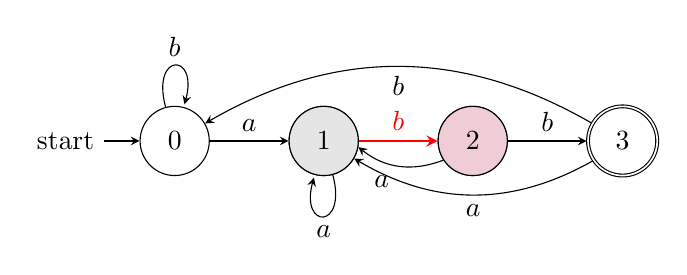
\begin{tikzpicture}[auto,
    ->,
    >=stealth
  ]
    \node[initial, state]   (0)                {$0$};
    \node[state]            (1) [right = of 0] {$1$};
    \node[state] (2) [right = of 1] {$2$};
    \node[state, accepting] (3) [right = of 2] {$3$};
    
    \path (0) edge[loop above] node {$b$} (0)
          (0) edge node {$a$} (1)
          (1) edge[loop below] node {$a$} (1)
          (1) edge[Red, thick] node {$b$} (2)
          (2) edge node {$b$} (3)
          (2) edge[bend left] node {$a$} (1.350)
          (3) edge[bend left] node {$a$} (1.330)
          (3) edge[bend right] node {$b$} (0)
    ;
        \node[state, fill=Gray!20]   (1a) at  (1)    {$1$};
        \node[state, fill=Pink!20]   (2a) at  (2)    {$2$};
  \end{tikzpicture}
}

\vspace{1cm}
\begin{tabular}{p{0.3\textwidth} @{\hspace{1cm}} c}
\textbf{Input:} $aa{\color{Red}\textbf{b}}babb$ &
\resizebox{0.6\textwidth}{!}{
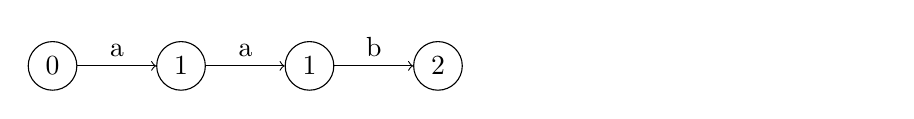
\begin{tikzpicture}
\node[circle, draw=Black] (s0) {0};
\node[circle, draw=Black, right=of s0] (s1) {1};
\node[circle, draw=Black, right=of s1] (s2) {1};
\node[circle, draw=Black, right=of s2] (s3) {2};
\node[circle, draw=none, right=of s3] (s4) {\ };
\node[circle, draw=none, right=of s4] (s5) {\ };
\node[circle, draw=none, right=of s5] (s6) {\ };
\node[circle, draw=none, right=of s6] (s7) { };

\draw[->] (s0) to node[above]{a} (s1);
\draw[->] (s1) to node[above]{a} (s2);
\draw[->] (s2) to node[above]{b} (s3);
%\draw[->] (s3) to node[above]{b} (s4);
%\draw[->] (s4) to node[above]{a} (s5);
%\draw[->] (s5) to node[above]{b} (s6);
%draw[->] (s6) to node[above]{b} (s7);
\end{tikzpicture}
}
\end{tabular}

\end{center}

\end{frame}
% frame end %%%%%%%%%%%%%%%%%%%%%%%%


% frame begin %%%%%%%%%%%%%%%%%%%%%%%%
\begin{frame}{Simulation of DFAs}

\myminorheader{Example 1}


\begin{center}
\resizebox{!}{0.2\textheight}{%
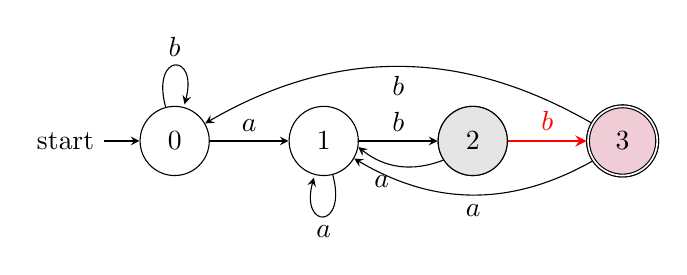
\begin{tikzpicture}[auto,
    ->,
    >=stealth
  ]
    \node[initial, state]   (0)                {$0$};
    \node[state]            (1) [right = of 0] {$1$};
    \node[state] (2) [right = of 1] {$2$};
    \node[state, accepting] (3) [right = of 2] {$3$};
    
    \path (0) edge[loop above] node {$b$} (0)
          (0) edge node {$a$} (1)
          (1) edge[loop below] node {$a$} (1)
          (1) edge node {$b$} (2)
          (2) edge[Red, thick] node {$b$} (3)
          (2) edge[bend left] node {$a$} (1.350)
          (3) edge[bend left] node {$a$} (1.330)
          (3) edge[bend right] node {$b$} (0)
    ;
        \node[state, fill=Gray!20]   (2a) at  (2)    {$2$};
        \node[state, accepting, fill=Pink!20]   (3a) at  (3)    {$3$};
  \end{tikzpicture}
}

\vspace{1cm}
\begin{tabular}{p{0.3\textwidth} @{\hspace{1cm}} c}
\textbf{Input:} $aab{\color{Red}\textbf{b}}abb$ &
\resizebox{0.6\textwidth}{!}{
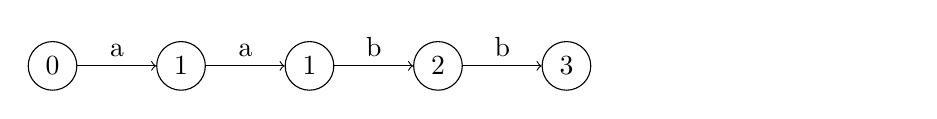
\begin{tikzpicture}
\node[circle, draw=Black] (s0) {0};
\node[circle, draw=Black, right=of s0] (s1) {1};
\node[circle, draw=Black, right=of s1] (s2) {1};
\node[circle, draw=Black, right=of s2] (s3) {2};
\node[circle, draw=Black, right=of s3] (s4) {3};
\node[circle, draw=none, right=of s4] (s5) {\ };
\node[circle, draw=none, right=of s5] (s6) {\ };
\node[circle, draw=none, right=of s6] (s7) { };

\draw[->] (s0) to node[above]{a} (s1);
\draw[->] (s1) to node[above]{a} (s2);
\draw[->] (s2) to node[above]{b} (s3);
\draw[->] (s3) to node[above]{b} (s4);
%\draw[->] (s4) to node[above]{a} (s5);
%\draw[->] (s5) to node[above]{b} (s6);
%draw[->] (s6) to node[above]{b} (s7);
\end{tikzpicture}
}
\end{tabular}

\end{center}

\end{frame}
% frame end %%%%%%%%%%%%%%%%%%%%%%%%

% frame begin %%%%%%%%%%%%%%%%%%%%%%%%
\begin{frame}{Simulation of DFAs}

\myminorheader{Example 1}


\begin{center}
\resizebox{!}{0.2\textheight}{%
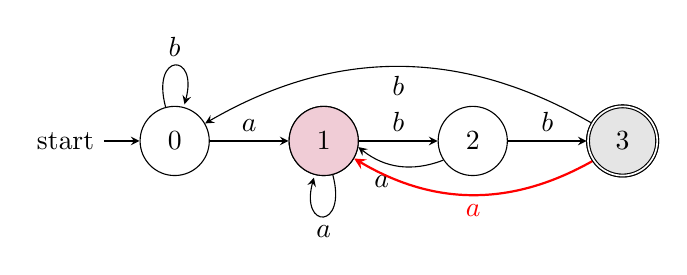
\begin{tikzpicture}[auto,
    ->,
    >=stealth
  ]
    \node[initial, state]   (0)                {$0$};
    \node[state]            (1) [right = of 0] {$1$};
    \node[state] (2) [right = of 1] {$2$};
    \node[state, accepting] (3) [right = of 2] {$3$};
    
    \path (0) edge[loop above] node {$b$} (0)
          (0) edge node {$a$} (1)
          (1) edge[loop below] node {$a$} (1)
          (1) edge node {$b$} (2)
          (2) edge node {$b$} (3)
          (2) edge[bend left] node {$a$} (1.350)
          (3) edge[Red, thick, bend left] node {$a$} (1.330)
          (3) edge[bend right] node {$b$} (0)
    ;
        \node[state, accepting, fill=Gray!20]   (3a) at  (3)    {$3$};
        \node[state, fill=Pink!20]   (1a) at  (1)    {$1$};
  \end{tikzpicture}
}

\vspace{1cm}
\begin{tabular}{p{0.3\textwidth} @{\hspace{1cm}} c}
\textbf{Input:} $aabb{\color{Red}\textbf{a}}bb$ &
\resizebox{0.6\textwidth}{!}{
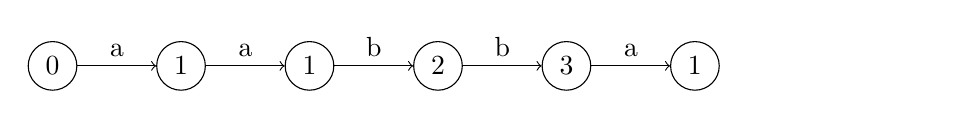
\begin{tikzpicture}
\node[circle, draw=Black] (s0) {0};
\node[circle, draw=Black, right=of s0] (s1) {1};
\node[circle, draw=Black, right=of s1] (s2) {1};
\node[circle, draw=Black, right=of s2] (s3) {2};
\node[circle, draw=Black, right=of s3] (s4) {3};
\node[circle, draw=Black, right=of s4] (s5) {1};
\node[circle, draw=none, right=of s5] (s6) {\ };
\node[circle, draw=none, right=of s6] (s7) { };

\draw[->] (s0) to node[above]{a} (s1);
\draw[->] (s1) to node[above]{a} (s2);
\draw[->] (s2) to node[above]{b} (s3);
\draw[->] (s3) to node[above]{b} (s4);
\draw[->] (s4) to node[above]{a} (s5);
%\draw[->] (s5) to node[above]{b} (s6);
%draw[->] (s6) to node[above]{b} (s7);
\end{tikzpicture}
}
\end{tabular}

\end{center}

\end{frame}
% frame end %%%%%%%%%%%%%%%%%%%%%%%%

% frame begin %%%%%%%%%%%%%%%%%%%%%%%%
\begin{frame}{Simulation of DFAs}

\myminorheader{Example 1}

\begin{center}
\resizebox{!}{0.2\textheight}{%
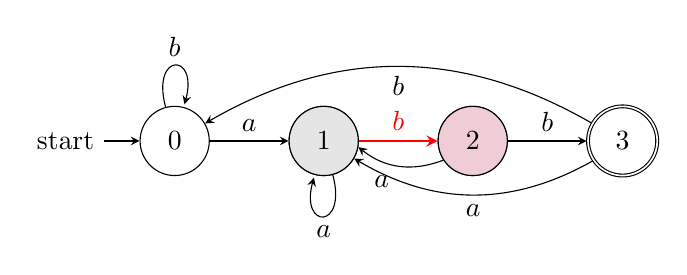
\begin{tikzpicture}[auto,
    ->,
    >=stealth
  ]
    \node[initial, state]   (0)                {$0$};
    \node[state]            (1) [right = of 0] {$1$};
    \node[state] (2) [right = of 1] {$2$};
    \node[state, accepting] (3) [right = of 2] {$3$};
    
    \path (0) edge[loop above] node {$b$} (0)
          (0) edge node {$a$} (1)
          (1) edge[loop below] node {$a$} (1)
          (1) edge[Red, thick] node {$b$} (2)
          (2) edge node {$b$} (3)
          (2) edge[bend left] node {$a$} (1.350)
          (3) edge[bend left] node {$a$} (1.330)
          (3) edge[bend right] node {$b$} (0)
    ;
        \node[state, fill=Gray!20]   (1a) at  (1)    {$1$};
        \node[state, fill=Pink!20]   (2a) at  (2)    {$2$};
  \end{tikzpicture}
}

\vspace{1cm}
\begin{tabular}{p{0.3\textwidth} @{\hspace{1cm}} c}
\textbf{Input:} $aabba{\color{Red}\textbf{b}}b$ &
\resizebox{0.6\textwidth}{!}{
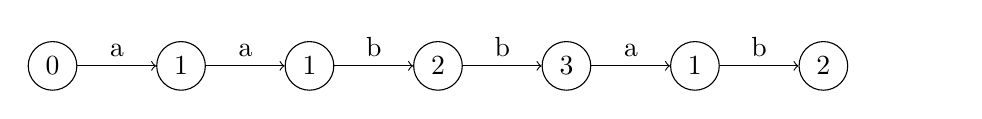
\begin{tikzpicture}
\node[circle, draw=Black] (s0) {0};
\node[circle, draw=Black, right=of s0] (s1) {1};
\node[circle, draw=Black, right=of s1] (s2) {1};
\node[circle, draw=Black, right=of s2] (s3) {2};
\node[circle, draw=Black, right=of s3] (s4) {3};
\node[circle, draw=Black, right=of s4] (s5) {1};
\node[circle, draw=Black, right=of s5] (s6) {2};
\node[circle, draw=none, right=of s6] (s7) {};

\draw[->] (s0) to node[above]{a} (s1);
\draw[->] (s1) to node[above]{a} (s2);
\draw[->] (s2) to node[above]{b} (s3);
\draw[->] (s3) to node[above]{b} (s4);
\draw[->] (s4) to node[above]{a} (s5);
\draw[->] (s5) to node[above]{b} (s6);
%draw[->] (s6) to node[above]{b} (s7);
\end{tikzpicture}
}
\end{tabular}

\end{center}

\end{frame}
% frame end %%%%%%%%%%%%%%%%%%%%%%%%


% frame begin %%%%%%%%%%%%%%%%%%%%%%%%
\begin{frame}{Simulation of DFAs}

\myminorheader{Example 1}

\begin{center}
\resizebox{!}{0.2\textheight}{%
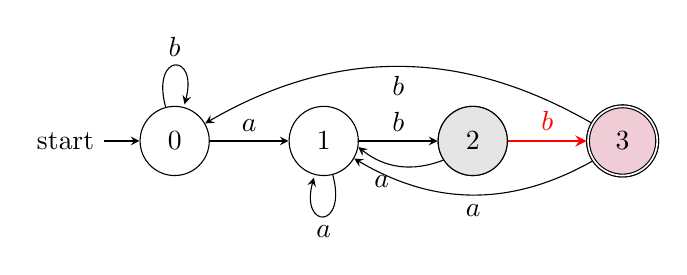
\begin{tikzpicture}[auto,
    ->,
    >=stealth
  ]
    \node[initial, state]   (0)                {$0$};
    \node[state]            (1) [right = of 0] {$1$};
    \node[state] (2) [right = of 1] {$2$};
    \node[state, accepting] (3) [right = of 2] {$3$};
    
    \path (0) edge[loop above] node {$b$} (0)
          (0) edge node {$a$} (1)
          (1) edge[loop below] node {$a$} (1)
          (1) edge node {$b$} (2)
          (2) edge[Red, thick] node {$b$} (3)
          (2) edge[bend left] node {$a$} (1.350)
          (3) edge[bend left] node {$a$} (1.330)
          (3) edge[bend right] node {$b$} (0)
    ;
    
        \node[state, fill=Gray!20]   (2a) at  (2)    {$2$};
        \node[state, accepting, fill=Pink!20]   (3a) at  (3)    {$3$};
  \end{tikzpicture}
}

\vspace{1cm}
\begin{tabular}{p{0.3\textwidth} @{\hspace{1cm}} c}
\textbf{Input:} $aabbab{\color{Red}\textbf{b}}$ &
\resizebox{0.6\textwidth}{!}{
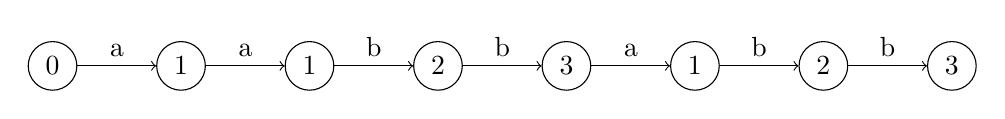
\begin{tikzpicture}
\node[circle, draw=Black] (s0) {0};
\node[circle, draw=Black, right=of s0] (s1) {1};
\node[circle, draw=Black, right=of s1] (s2) {1};
\node[circle, draw=Black, right=of s2] (s3) {2};
\node[circle, draw=Black, right=of s3] (s4) {3};
\node[circle, draw=Black, right=of s4] (s5) {1};
\node[circle, draw=Black, right=of s5] (s6) {2};
\node[circle, draw=Black, right=of s6] (s7) {3};

\draw[->] (s0) to node[above]{a} (s1);
\draw[->] (s1) to node[above]{a} (s2);
\draw[->] (s2) to node[above]{b} (s3);
\draw[->] (s3) to node[above]{b} (s4);
\draw[->] (s4) to node[above]{a} (s5);
\draw[->] (s5) to node[above]{b} (s6);
\draw[->] (s6) to node[above]{b} (s7);
\end{tikzpicture}
}
\end{tabular}

\end{center}


\end{frame}
% frame end %%%%%%%%%%%%%%%%%%%%%%%%


% frame begin %%%%%%%%%%%%%%%%%%%%%%%%
\begin{frame}{Simulation of DFAs}

\myminorheader{Example 2}

\begin{center}
\resizebox{!}{0.2\textheight}{%
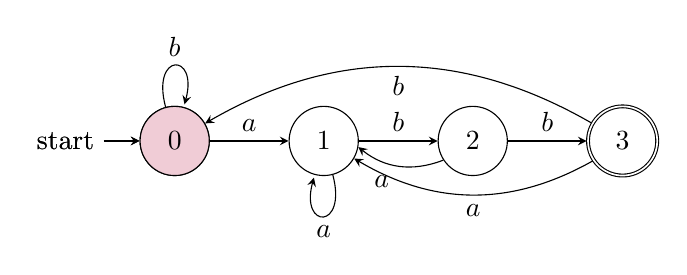
\begin{tikzpicture}[auto,
    ->,
    >=stealth
  ]
    \node[initial, state]   (0)                {$0$};
    \node[state]            (1) [right = of 0] {$1$};
    \node[state] (2) [right = of 1] {$2$};
    \node[state, accepting] (3) [right = of 2] {$3$};
    
    \path (0) edge[loop above] node {$b$} (0)
          (0) edge node {$a$} (1)
          (1) edge[loop below] node {$a$} (1)
          (1) edge node {$b$} (2)
          (2) edge node {$b$} (3)
          (2) edge[bend left] node {$a$} (1.350)
          (3) edge[bend left] node {$a$} (1.330)
          (3) edge[bend right] node {$b$} (0)
    ;
    
        \node[initial, state, fill=Pink!20]   (0a) at  (0)    {$0$};
  \end{tikzpicture}
}

\vspace{1cm}
\begin{tabular}{p{0.3\textwidth} @{\hspace{1cm}} c}
\textbf{Input:} $abab$ &
\resizebox{0.6\textwidth}{!}{
\begin{tikzpicture}
\node[circle, draw=Black] (s0) {0};
\node[circle, draw=none, right=of s0] (s1) {\ };
\node[circle, draw=none, right=of s1] (s2) {\ };
\node[circle, draw=none, right=of s2] (s3) {\ };
\node[circle, draw=none, right=of s3] (s4) {\ };

%\draw[->] (s0) to node[above]{a} (s1);
%\draw[->] (s1) to node[above]{b} (s2);
%\draw[->] (s2) to node[above]{a} (s3);
%\draw[->] (s3) to node[above]{b} (s4);
\end{tikzpicture}
}
\end{tabular}

\end{center}


\end{frame}
% frame end %%%%%%%%%%%%%%%%%%%%%%%%

% frame begin %%%%%%%%%%%%%%%%%%%%%%%%
\begin{frame}{Simulation of DFAs}

\myminorheader{Example 2}

\begin{center}
\resizebox{!}{0.2\textheight}{%
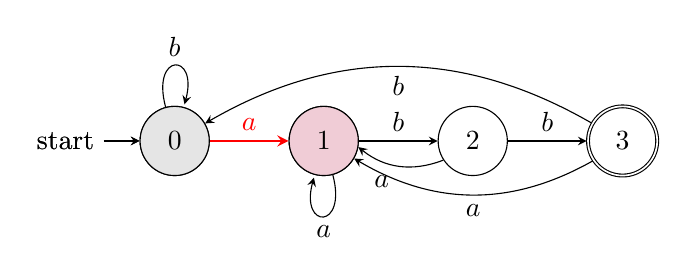
\begin{tikzpicture}[auto,
    ->,
    >=stealth
  ]
    \node[initial, state]   (0)                {$0$};
    \node[state]            (1) [right = of 0] {$1$};
    \node[state] (2) [right = of 1] {$2$};
    \node[state, accepting] (3) [right = of 2] {$3$};
    
    \path (0) edge[loop above] node {$b$} (0)
          (0) edge[Red, thick] node {$a$} (1)
          (1) edge[loop below] node {$a$} (1)
          (1) edge node {$b$} (2)
          (2) edge node {$b$} (3)
          (2) edge[bend left] node {$a$} (1.350)
          (3) edge[bend left] node {$a$} (1.330)
          (3) edge[bend right] node {$b$} (0)
    ;
    
        \node[initial, state, fill=Gray!20]   (0a) at  (0)    {$0$};
        \node[state, fill=Pink!20]   (1a) at  (1)    {$1$};
  \end{tikzpicture}
}

\vspace{1cm}
\begin{tabular}{p{0.3\textwidth} @{\hspace{1cm}} c}
\textbf{Input:} ${\color{Red}\textbf{a}}bab$ &
\resizebox{0.6\textwidth}{!}{
\begin{tikzpicture}
\node[circle, draw=Black] (s0) {0};
\node[circle, draw=Black, right=of s0] (s1) {1};
\node[circle, draw=none, right=of s1] (s2) {\ };
\node[circle, draw=none, right=of s2] (s3) {\ };
\node[circle, draw=none, right=of s3] (s4) {\ };

\draw[->] (s0) to node[above]{a} (s1);
%\draw[->] (s1) to node[above]{b} (s2);
%\draw[->] (s2) to node[above]{a} (s3);
%\draw[->] (s3) to node[above]{b} (s4);
\end{tikzpicture}
}
\end{tabular}

\end{center}


\end{frame}
% frame end %%%%%%%%%%%%%%%%%%%%%%%%

% frame begin %%%%%%%%%%%%%%%%%%%%%%%%
\begin{frame}{Simulation of DFAs}

\myminorheader{Example 2}

\begin{center}
\resizebox{!}{0.2\textheight}{%
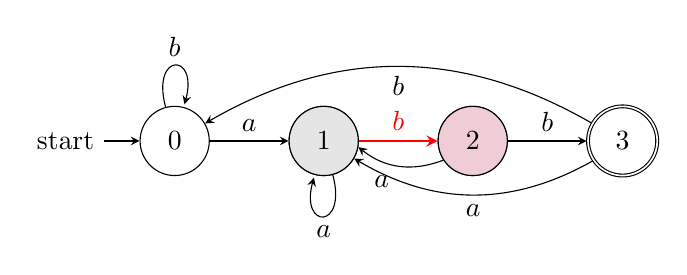
\begin{tikzpicture}[auto,
    ->,
    >=stealth
  ]
    \node[initial, state]   (0)                {$0$};
    \node[state]            (1) [right = of 0] {$1$};
    \node[state] (2) [right = of 1] {$2$};
    \node[state, accepting] (3) [right = of 2] {$3$};
    
    \path (0) edge[loop above] node {$b$} (0)
          (0) edge node {$a$} (1)
          (1) edge[loop below] node {$a$} (1)
          (1) edge[Red, thick] node {$b$} (2)
          (2) edge node {$b$} (3)
          (2) edge[bend left] node {$a$} (1.350)
          (3) edge[bend left] node {$a$} (1.330)
          (3) edge[bend right] node {$b$} (0)
    ;
    
        \node[state, fill=Gray!20]   (1a) at  (1)    {$1$};
        \node[state, fill=Pink!20]   (3a) at  (2)    {$2$};
  \end{tikzpicture}
}

\vspace{1cm}
\begin{tabular}{p{0.3\textwidth} @{\hspace{1cm}} c}
\textbf{Input:} $a{\color{Red}\textbf{b}}ab$ &
\resizebox{0.6\textwidth}{!}{
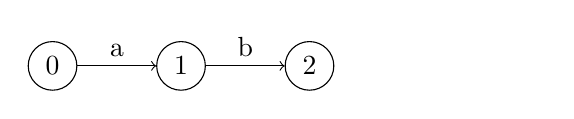
\begin{tikzpicture}
\node[circle, draw=Black] (s0) {0};
\node[circle, draw=Black, right=of s0] (s1) {1};
\node[circle, draw=Black, right=of s1] (s2) {2};
\node[circle, draw=none, right=of s2] (s3) {\ };
\node[circle, draw=none, right=of s3] (s4) {\ };

\draw[->] (s0) to node[above]{a} (s1);
\draw[->] (s1) to node[above]{b} (s2);
%\draw[->] (s2) to node[above]{a} (s3);
%\draw[->] (s3) to node[above]{b} (s4);
\end{tikzpicture}
}
\end{tabular}

\end{center}


\end{frame}
% frame end %%%%%%%%%%%%%%%%%%%%%%%%

% frame begin %%%%%%%%%%%%%%%%%%%%%%%%
\begin{frame}{Simulation of DFAs}

\myminorheader{Example 2}

\begin{center}
\resizebox{!}{0.2\textheight}{%
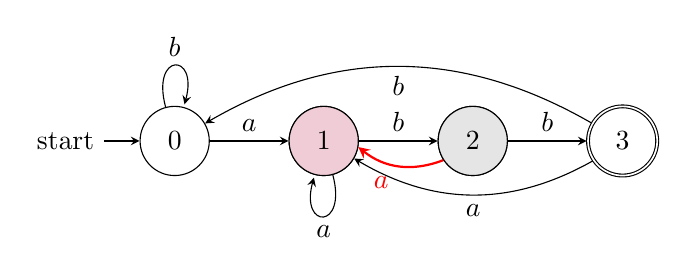
\begin{tikzpicture}[auto,
    ->,
    >=stealth
  ]
    \node[initial, state]   (0)                {$0$};
    \node[state]            (1) [right = of 0] {$1$};
    \node[state] (2) [right = of 1] {$2$};
    \node[state, accepting] (3) [right = of 2] {$3$};
    
    \path (0) edge[loop above] node {$b$} (0)
          (0) edge node {$a$} (1)
          (1) edge[loop below] node {$a$} (1)
          (1) edge node {$b$} (2)
          (2) edge node {$b$} (3)
          (2) edge[Red, thick, bend left] node {$a$} (1.350)
          (3) edge[bend left] node {$a$} (1.330)
          (3) edge[bend right] node {$b$} (0)
    ;
    
        \node[state, fill=Gray!20]   (2a) at  (2)    {$2$};
        \node[state, fill=Pink!20]   (1a) at  (1)    {$1$};
  \end{tikzpicture}
}

\vspace{1cm}
\begin{tabular}{p{0.3\textwidth} @{\hspace{1cm}} c}
\textbf{Input:} $ab{\color{Red}\textbf{a}}b$ &
\resizebox{0.6\textwidth}{!}{
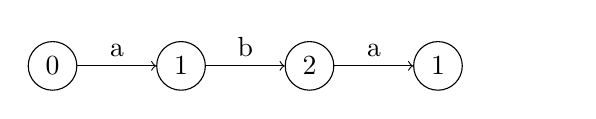
\begin{tikzpicture}
\node[circle, draw=Black] (s0) {0};
\node[circle, draw=Black, right=of s0] (s1) {1};
\node[circle, draw=Black, right=of s1] (s2) {2};
\node[circle, draw=Black, right=of s2] (s3) {1};
\node[circle, draw=none, right=of s3] (s4) {\ };

\draw[->] (s0) to node[above]{a} (s1);
\draw[->] (s1) to node[above]{b} (s2);
\draw[->] (s2) to node[above]{a} (s3);
%\draw[->] (s3) to node[above]{b} (s4);
\end{tikzpicture}
}
\end{tabular}

\end{center}


\end{frame}
% frame end %%%%%%%%%%%%%%%%%%%%%%%%

% frame begin %%%%%%%%%%%%%%%%%%%%%%%%
\begin{frame}{Simulation of DFAs}

\myminorheader{Example 2}

\begin{center}
\resizebox{!}{0.2\textheight}{%
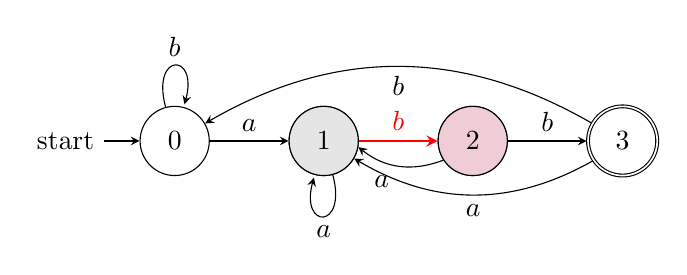
\begin{tikzpicture}[auto,
    ->,
    >=stealth
  ]
    \node[initial, state]   (0)                {$0$};
    \node[state]            (1) [right = of 0] {$1$};
    \node[state] (2) [right = of 1] {$2$};
    \node[state, accepting] (3) [right = of 2] {$3$};
    
    \path (0) edge[loop above] node {$b$} (0)
          (0) edge node {$a$} (1)
          (1) edge[loop below] node {$a$} (1)
          (1) edge[Red, thick] node {$b$} (2)
          (2) edge node {$b$} (3)
          (2) edge[bend left] node {$a$} (1.350)
          (3) edge[bend left] node {$a$} (1.330)
          (3) edge[bend right] node {$b$} (0)
    ;
    
        \node[state, fill=Gray!20]   (1a) at  (1)    {$1$};
        \node[state, fill=Pink!20]   (2a) at  (2)    {$2$};
  \end{tikzpicture}
}

\vspace{1cm}
\begin{tabular}{p{0.3\textwidth} @{\hspace{1cm}} c}
\textbf{Input:} $aba{\color{Red}\textbf{b}}$ &
\resizebox{0.6\textwidth}{!}{
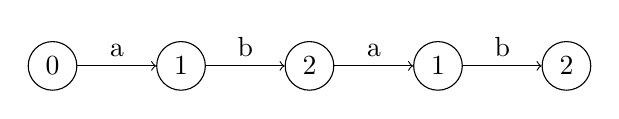
\begin{tikzpicture}
\node[circle, draw=Black] (s0) {0};
\node[circle, draw=Black, right=of s0] (s1) {1};
\node[circle, draw=Black, right=of s1] (s2) {2};
\node[circle, draw=Black, right=of s2] (s3) {1};
\node[circle, draw=Black, right=of s3] (s4) {2};

\draw[->] (s0) to node[above]{a} (s1);
\draw[->] (s1) to node[above]{b} (s2);
\draw[->] (s2) to node[above]{a} (s3);
\draw[->] (s3) to node[above]{b} (s4);
\end{tikzpicture}
}
\end{tabular}

\end{center}


\end{frame}
% frame end %%%%%%%%%%%%%%%%%%%%%%%%

\end{document}
